
\documentclass[twoside,twocolumn]{article}
\usepackage{amsmath}
\usepackage{blindtext} % Package to generate dummy text throughout this template 
\usepackage{graphicx}
\usepackage{natbib}

\usepackage[sc]{mathpazo} % Use the Palatino font
\usepackage[T1]{fontenc} % Use 8-bit encoding that has 256 glyphs
\linespread{1.05} % Line spacing - Palatino needs more space between lines
\usepackage{microtype} % Slightly tweak font spacing for aesthetics

\usepackage[english]{babel} % Language hyphenation and typographical rules

\usepackage[hmarginratio=1:1,top=32mm,columnsep=20pt]{geometry} % Document margins
\usepackage[hang, small,labelfont=bf,up,textfont=it,up]{caption} % Custom captions under/above floats in tables or figures
\usepackage{booktabs} % Horizontal rules in tables

\usepackage{lettrine} % The lettrine is the first enlarged letter at the beginning of the text

\usepackage{enumitem} % Customized lists
\setlist[itemize]{noitemsep} % Make itemize lists more compact

\usepackage{abstract} % Allows abstract customization
\renewcommand{\abstractnamefont}{\normalfont\bfseries} % Set the "Abstract" text to bold
\renewcommand{\abstracttextfont}{\normalfont\small\itshape} % Set the abstract itself to small italic text

\usepackage{titlesec} % Allows customization of titles
\renewcommand\thesection{\Roman{section}} % Roman numerals for the sections
\renewcommand\thesubsection{\roman{subsection}} % roman numerals for subsections
\titleformat{\section}[block]{\large\scshape\centering}{\thesection.}{1em}{} % Change the look of the section titles
\titleformat{\subsection}[block]{\large}{\thesubsection.}{1em}{} % Change the look of the section titles

\usepackage{fancyhdr} % Headers and footers
\pagestyle{fancy} % All pages have headers and footers
\fancyhead{} % Blank out the default header
\fancyfoot{} % Blank out the default footer
\fancyhead[C]{FYS4150 $\bullet$ Project 1 $\bullet$ September 2016} % Custom header text
\fancyfoot[RO,LE]{\thepage} % Custom footer text

\usepackage{titling} % Customizing the title section

\usepackage{hyperref} % For hyperlinks in the PDF

%----------------------------------------------------------------------------------------
%	TITLE SECTION
%----------------------------------------------------------------------------------------

\setlength{\droptitle}{-4\baselineskip} % Move the title up

\pretitle{\begin{center}\Huge\bfseries} % Article title formatting
\posttitle{\end{center}} % Article title closing formatting
\title{FYS4150 - Project 1} % Article title
\author{%
\textsc{Heine H. Ness \& Sindre R. Bilden}\thanks{A thank you or further information} \\[1ex] % Your name
\normalsize University of Oslo \\ % Your institution
\normalsize \href{mailto:h.h.ness@fys.uio.no}{h.h.ness@fys.uio.no}\ ; \href{mailto:s.r.bilden@fys.uio.no}{s.r.bilden@fys.uio.no}\\% Your email address
\normalsize \href{https://github.com/sindrerb/FYS4150-Collaboration}{github.com/sindrerb/FYS4150-Collaboration}
%\and % Uncomment if 2 authors are required, duplicate these 4 lines if more
%\textsc{Jane Smith}\thanks{Corresponding author} \\[1ex] % Second author's name
%\normalsize University of Utah \\ % Second author's institution
%\normalsize \href{mailto:jane@smith.com}{jane@smith.com} % Second author's email address
}
\date{\today} % Leave empty to omit a date
\renewcommand{\maketitlehookd}{%
\begin{abstract}
\noindent \blindtext % Dummy abstract text - replace \blindtext with your abstract text
\end{abstract}
}

\newcommand{\nl}{

\medskip
\noindent
}

%----------------------------------------------------------------------------------------

\begin{document}

% Print the title
\maketitle

%----------------------------------------------------------------------------------------
%	ARTICLE CONTENTS
%----------------------------------------------------------------------------------------

\section{Introduction}

\lettrine[nindent=0em,lines=3]{T}his project will examinate different techniques for approximating the solution to a differential equation where a continious function is known. The equation describes an electrostatic potential $\Phi$ generated by a localized charge density $\rho(\vec{r})$ and is usualy described - in three dimentions - by:
\begin{equation}
\nabla^2\Phi = -4\pi \rho(\vec{r}) \label{eq:Poisson3D}
\end{equation}
If $\rho(\vec{r})$ is spherical symmetric, eq. \ref{eq:Poisson3D} may be written in a one-dimentional manner by substituting $\phi(r)=r\Phi(r)$:
\begin{equation}
\frac{d^2\phi(r)}{dr^2}=-4\pi r\rho(r) \label{eq:Poisson1D}
\end{equation}
By rewriting eq. \ref{eq:Poisson1D} to a general form it reads:
\begin{equation}
-u''(x)=f(x)
\end{equation}
In this spesific case, the Poisson equation is solved by \textit{Gaussian elimination} of a set of linear equations, both in a general manner and an optimized way of a spesific matrix. The optimized method is later compared with another general method called \textit{LU-decomposition}.

%------------------------------------------------

\section{Methods}
The methods used in this projects are the following:
\begin{itemize}
\item Dirichlet boundary conditions
\item Nummerical derivation
\item Gaussian elimination
\item LU-decomposition
\end{itemize}

\subsection{Dirichlet boundary condition}
Dirichlet boundary conditions - also refered to as fixed boundary condition - specifies the value of a given function on a surface $T=f(r,t)$. In a one-dimentional problem it translates to defining an interval of $x$ - $x\in [x_{min},x_{max}]$ - and the function values $f(x_{min})=f_l$ and $f(x_{max})=f_h$ at the edges of the intervall.

\subsection{Nummerical derivarion}
The derivative of a discrete funtion may be found by nummerical derivation. The principle of nummerical derivation is a result of Taylor expansion. By expanding a function from   a point $x$ with a step $h$, two equations form depending on the direction:
\begin{equation}
f(x+h) = f(x)+hf'(x)+\frac{h^2}{2}f''(x)\ldots \label{eq:taylor_pos}
\end{equation}
\begin{equation}
f(x-h) = f(x)-hf'(x)+\frac{h^2}{2}f''(x)\ldots \label{eq:taylor_neg}
\end{equation}
By adding eq. \ref{eq:taylor_neg} to eq. \ref{eq:taylor_pos}, a approximation for the second derivative is achieved.
\begin{equation}
f'' = \frac{f_+-2f+f_-}{h^2}+\frac{h^4}{6h^2}f^{\mathit{IV}}\label{eq:sec_der}
\end{equation}
Where $f_+ = f(x+h)$, $f=f(x)$, $f_-=f(x-h)$ and $f^{IV}$ is the fourth derivative of $f(x)$. By truncating the series at the fourth derivative a small mathematical error - $\mathcal{O}$ - appears in the order of $h^2$. If a discrete funtion is introduced where $f_i = f(x_i) = f(c_0+ih)$, eq. \ref{eq:sec_der} may be rewritten to an algorithm for the nummerical second derivative.
\begin{equation}
f''_i = \frac{f_{i+1}-2f_i+f_{i-1}}{h^2}\label{eq:sec_der_discrete}
\end{equation}
In eq. \ref{eq:sec_der_discrete} the mathematical error $\mathcal{O}(h^2)$ is neglected.

\subsection{Thomas algorithm}
Thomas algorithm is a variant of Gaussian elimination used on tridiagonal matrices [kilde], where Gaussian elimination is a method for simplifying a set of $N$ linear equations with $n$ unknown variables $x_i$ $i=0,1,\ldots,n-1$. Thomas algorithm is usefull if the equations is on the form 
\begin{align*}
a_{i}x_{i-1}+b_{i}x_i+c_{i}x_{i+1}&=y_i
\end{align*}
Resulting in a matrix equation $Ax= y$ where $A$ and $y$ is known.
\begin{equation*}
\begin{bmatrix}
b_1&c_1&0&\cdots &0\\
a_2&b_2&c_2& \ddots & \vdots\\
0&a_3&b_3&\ddots&0\\
\vdots&\ddots&\ddots&\ddots&c_{n-1}\\
0&\cdots&0&a_n&b_n
\end{bmatrix}
\begin{bmatrix}
x_1\\x_2\\x_3\\x_4\\\vdots\\x_{n}
\end{bmatrix}=
\begin{bmatrix}
y_1\\y_2\\y_3\\y_4\\\vdots\\y_{n}
\end{bmatrix} 
\end{equation*}
Both Thomas algoritm and Gaussian elimination is divided into two main parts, forward and backward substitution.
\subsubsection{Forward substitution}
The forward substitution is focusing on reducing the number of elements in a column to a minimum. In other words, row reduction is first used on the matrix $A$ to eliminate all elements $a_{i}$. Turning the matrix equation to $Bx=\hat{y}$:
\begin{equation*}
\begin{bmatrix}
b_1&c_1&0&\cdots &0\\
0&\tilde{b}_2&c_2& \ddots & \vdots\\
0&0&\tilde{b}_3&\ddots&0\\
\vdots&\ddots&\ddots&\ddots&c_{n-1}\\
0&\cdots&0&0&\tilde{b}_n
\end{bmatrix}
\begin{bmatrix}
x_1\\x_2\\x_3\\x_4\\\vdots\\x_{n}
\end{bmatrix}=
\begin{bmatrix}
\tilde{y}_1\\\tilde{y}_2\\\tilde{y}_3\\\tilde{y}_4\\\vdots\\\tilde{y}_{n}
\end{bmatrix} 
\end{equation*}
where $\tilde{b}$ and $\tilde{y}$ is affected by the row reduction. The new set of linear equations is the basis for backward substitution.
\subsubsection{Backward substitution}
The concept of backwars substitution is to solve the the set of equations from bottom to top. The bottom $x$ can be expressed as $x_n=\frac{\tilde{y}_n}{\tilde{b}_n}$ and may be used in the equation above. In the end, all elements of $x$ is known. In total, the Thomas algoritm is using $9n$ floating point operations (FLOPS). If the matrix elements is constant through every diagonal, the number of FLOPS may be reduced to $4n$.

\subsection{LU-decompostition}


\subsection{Numerical error estimate}

Since we are using numerical derivation this gives us an approximation to the analytical answer.
Therfore it is interesting to see how good our approximation is.    
A good way to do this is to look at the difference between the two.
\nl
At small step lenghts ($h$) we will have a good approximation if the theori is correct and therfore it is convenient too look at the logaritme of the difference we also use the absolute walue since we dont care if we are over or under the analytical answer. To avoid the logaritme of zero we also devide by the analytical value.
\nl
So we get the relative error $\varepsilon$ and for each step ve get:

\begin{equation}
\varepsilon_i = log\left(\left|\frac{u_i - v_i}{v_i}\right|\right)
\end{equation}

Here $u_i$ is the numerical value and $v_i$ is the analytical value at step $i$. And $log$ is the base 10 logaritme.

\section{Implementation}
By discretizing the simplified and generalized Poiison equation (eq. \ref{eq:sec_der}) in steps of $h$, we may approximate eq. \ref{eq:sec_der} with eq. \ref{eq:sec_der_num} where $v_i$ is the discrete values of the continium $u(x)$.
\begin{equation}
-\frac{v_{i+1}-2v_i+v_{i-1}}{h^2}=f_i \label{eq:sec_der_num}
\end{equation}
The equation may be rewritten into a linear equation
\begin{equation*}
av_{i-1}+bv_i+cv_{i+1}=\tilde{b}_i 
\end{equation*}
where $a=-1$, $b=2$, $c=-1$ and $\tilde{b}_i=f_ih^2$. By introducing dirichlet boundary conditions, $v_0=v_{n+1}=0$, the linear equations may be written in terms of matrix multiplication without loss of information. This results in $Av=\tilde{b}$:
\begin{equation}
\begin{bmatrix}
b&c&0&0&\cdots &0\\
a&b&c&0& \cdots & 0\\
0&a&b&c& \cdots & 0\\
\vdots&\vdots&\vdots&\vdots&\ddots&c\\
0&0&0&0&a&b
\end{bmatrix}
\begin{bmatrix}
v_1\\v_2\\\vdots\\v_{n-1}\\v_{n}
\end{bmatrix}=
\begin{bmatrix}
\tilde{b}_0\\\tilde{b}_1\\\vdots\\\tilde{b}_{n-2}\\\tilde{b}_{n-1}
\end{bmatrix} \label{eq:problem}
\end{equation}
The problem is now solvable by both Thomas algorithm and LU-decomposition. Since matrix $A$ has a constant value along it's diagonals, an optimized Thomas algorithm was constructed to this spesific matrix. All codes are tested with a reference function $f(x)$ with the known solution $u(x)$ where
\begin{equation*}
f(x)=100\exp[-10x]
\end{equation*}
\begin{equation*}
u(x)=1-\exp[-10]x-10\exp[-10x]
\end{equation*}
For all programs, divided in task $b$, $c$ and $d$ see the github repository: 

\begin{center}
 \href{https://github.com/sindrerb/FYS4150-Collaboration}{github.com/sindrerb/FYS4150-Collaboration}
\end{center}

\section{Results}
\subsection{LU-decomposition}
Solving eq. \ref{eq:problem} using LU-decomposition is a time consuming process. Even though the method reduces the numper of 
\subsection{General Thomas algorithm}
Solving eq. \ref{eq:problem} using Thomas algorithm gave a - by eye - satisfying approximation with 100 iterations, as seen in Figure \ref{fig:Thomas1E2}. The algorithm seems to has a tendency to underestimate the derivative and will approach exact solution from below, as seen in Figure \ref{fig:Thomas10}.

\begin{figure}[htp]
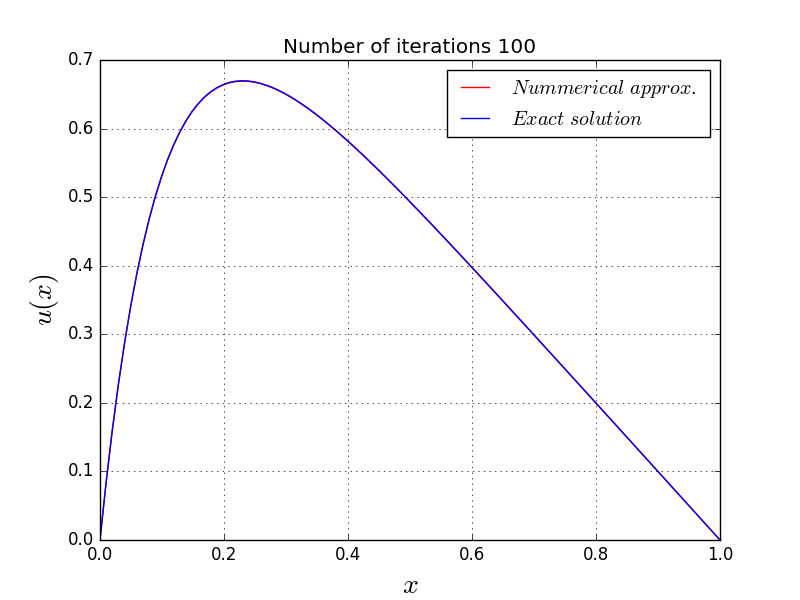
\includegraphics[width=0.5\textwidth]{./figures/b-run1e2.png} 
\caption{Plot of the nummerical approximation of $u(x)$ - in red - with 100 iterations by Thomas algorithm, compared to the exact solution $u(x)$ in blue.} \label{fig:Thomas1E2}
\end{figure}

\begin{figure}[htp]
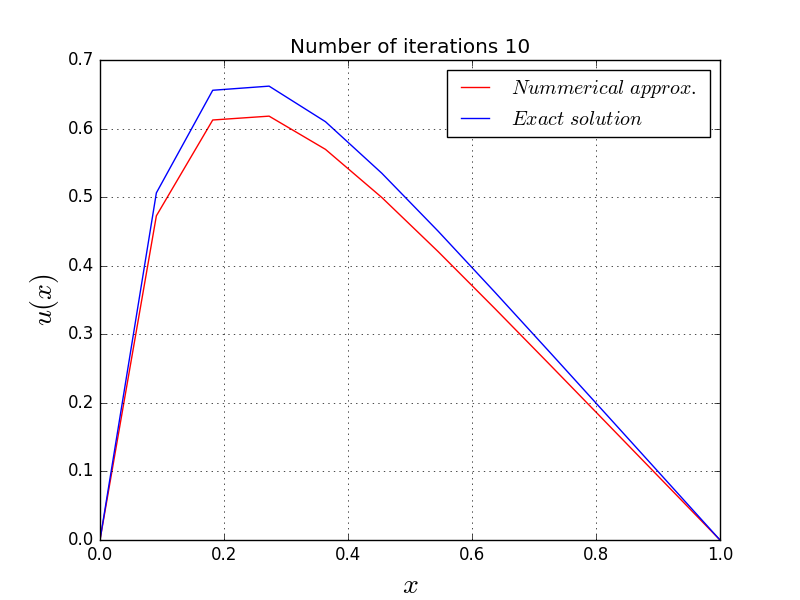
\includegraphics[width=0.5\textwidth]{./figures/b-run10.png} 
\caption{Plot of the nummerical approximation of $u(x)$ - in red - with 10 iterations by Thomas algorithm, compared to the exact solution $u(x)$ in blue.} \label{fig:Thomas10}
\end{figure}

\subsection{Specialized Thomas algorithm}
Solving eq. \ref{eq:problem} with a specialized Thomas algorithm gave the same results as the general algorithm, but reduced the number floating operations from $9n$ in the general algorithm to $4n$ in the specialized algorithm. The reduction in number of floating operations shorted the comutation time. A difference is hard to spot at a low numer of iterations, but higher number of iterations reveals a difference. A comparation of the timeusage by the two algorithms is found in Table \ref{tbl:ThompsonTime}.
\begin{table}[htp]
\centering
\begin{tabular}{|l|l|l|} \hline
Iterations & \multicolumn{2}{|c|}{Timeusage [s]}\\ \hline
 	& General 	& Special\\ \hline
1e1	& 1.0e-6	& 1.0E-6\\
1e2 & 9.0e-6	& 5.0e-6\\
1e3 & 5.1e-5	& 4.5e-5\\
1e4 & 7.66e-4	& 7.95e-4\\
1e5 & 5.021e-3	& 3.075e-3\\
1e6 & 2.6094e-2	&2.277e-2\\
1e7 & 2.7316e-1	& 2.26463e-1 \\ \hline
\end{tabular}
\caption{Table showing timeusage - in seconds - by the special and the general Thomson algorithm for a set of iterations.} \label{tbl:ThompsonTime}
\end{table}



\begin{table}[htp]
\centering
\begin{tabular}{|l|l|} \hline
Iterations & Relative error\\ \hline
1e1 & 1e(-1.17970)\\
1e2 & 1e(-3.08804)\\
1e3 & 1e(-5.08005)\\
1e4 & 1e(-7.07927)\\
1e5 & 1e(-9.07909)\\
1e6 & 1e(-10.7943)\\
1e7 & 1e(-9.54215)\\ \hline
\end{tabular}
\caption{Table showing the relative error for a set op iterations.}
\end{table}

\end{document}